\documentclass[14pt,aspectratio=1610]{beamer}

\usepackage[brazil]{babel}
\usepackage[utf8]{inputenc}
%\UseRawInputEncoding
\usepackage[T1]{fontenc}
%\usepackage{Sweave}
\usepackage{animate}
\usepackage{amsbsy}
\usepackage{amsfonts}
\usepackage{amsmath}
\usepackage{amssymb}
\usepackage{amsthm}
\usepackage[toc,page,title,titletoc]{appendix}
%\usepackage[fixlanguage]{babelbib}
%\usepackage[pdftex]{color}
\usepackage{dsfont}
\usepackage{esvect}
\usepackage[labelfont=bf]{caption}
\usepackage{subcaption}
\usepackage{float}
\usepackage[Glenn]{fncychap}%Sonny %Conny %Lenny %Glenn %Renje %Bjarne %Bjornstrup
%\usepackage{geometry, calc, color, setspace}%
%\geometry{a4paper, headsep=1.0cm, footskip=1cm, lmargin=3cm, rmargin=2cm, tmargin=3cm, bmargin=2cm}
\usepackage{graphicx}
\usepackage{indentfirst}%Para indentar os parágrafos automáticamente
\usepackage{lipsum}
\usepackage{longtable}
\usepackage{mathtools}
\usepackage{listings}%Inserir codigo do R no latex
\usepackage{multirow}
\usepackage{multicol}
\usepackage{csquotes}
\usepackage[style=authoryear,
			%style = bwl-FU,
			maxcitenames = 2,
			terseinits = true,
			natbib = true, 
			maxbibnames = 99]{biblatex}
\addbibresource{Referencias/Referencias.bib}
%\usepackage{csquotes}
%\usepackage[natbib=true,style=abnt, sorting=none]{biblatex}
%\addbibresource{bibliografia.bib}
\usepackage[figuresright]{rotating}
\usepackage{spalign}
%\usepackage{pgfpages}
\usepackage{pgfplots}
\pgfplotsset{compat=1.18}
\usepackage{tikz}
\usepackage{color, colortbl}
\usepackage{ragged2e}%para justificar o texto dentro de algum ambiente
\definecolor{Gray}{gray}{0.9}
\definecolor{LightCyan}{rgb}{0.88,1,1}
%\usepackage{grffile}

\usepackage[all]{xy}



\usetheme{Madrid}
\usecolortheme[RGB={193,0,0}]{structure}

%\setbeamertemplate{footline}[frame number]
%\setbeamertemplate{footline}[text line]{%
%  \parbox{\linewidth}{\vspace*{-8pt}\hfill\date{}\hfill\insertshortauthor\hfill\insertpagenumber}}
\beamertemplatenavigationsymbolsempty
\renewcommand{\vec}[1]{\mbox{\boldmath$#1$}}
\newtheorem{Teorema}{Teorema}
\newtheorem{Proposicao}{Proposição}
\newtheorem{Definicao}{Definição}
\newtheorem{Corolario}{Corolário}
\newtheorem{Demonstracao}{Demonstração}
\newcommand{\bx}{\ensuremath{\bar{x}}}
\newcommand{\Ho}{\ensuremath{H_{0}}}
\newcommand{\Hi}{\ensuremath{H_{1}}}
\everymath{\displaystyle}

\apptocmd{\frame}{}{\justifying}{} % Allow optional arguments after frame.

\title{Iniciação à Estatística}
\author{Prof. Fernando de Souza Bastos \texorpdfstring{\\ fernando.bastos@ufv.br}{}}
\institute{Departamento de Estatística \texorpdfstring{\\ Universidade Federal de Viçosa}{}\texorpdfstring{\\ Campus UFV - Viçosa}{}}
\date{}
\newcommand\mytext{Aula 2}
\newcommand\mytextt{Fernando de Souza Bastos}
\newcommand\mytexttt{\url{https://ufvest.github.io/}}

\makeatletter
\setbeamertemplate{footline}
{
  \leavevmode%
  \hbox{%
  \begin{beamercolorbox}[wd=.3\paperwidth,ht=2.25ex,dp=1ex,center]{author in head/foot}%
    \usebeamerfont{author in head/foot}\mytext
  \end{beamercolorbox}%
  \begin{beamercolorbox}[wd=.3\paperwidth,ht=2.25ex,dp=1ex,center]{title in head/foot}%
    \usebeamerfont{title in head/foot}\mytextt
  \end{beamercolorbox}%
  \begin{beamercolorbox}[wd=.35\paperwidth,ht=2.25ex,dp=1ex,right]{site in head/foot}%
    \usebeamerfont{site in head/foot}\mytexttt\hspace*{2em}
    \insertframenumber{} / \inserttotalframenumber\hspace*{2ex} 
  \end{beamercolorbox}}%
  \vskip0pt%
}
\makeatother

\providecommand{\arcsin}{} \renewcommand{\arcsin}{\hspace{2pt}\textrm{arcsen}}
\providecommand{\sin}{} \renewcommand{\sin}{\hspace{2pt}\textrm{sen}}
%\newtheorem{Teorema}{Teorema}
%\newtheorem{Proposicao}{Proposição}
%\newtheorem{Definicao}{Definição}
%\newtheorem{Corolario}{Corolário}
%\newtheorem{Demonstracao}{Demonstração}

\titlegraphic{\hspace*{8cm}\href{https://fsbmat-ufv.github.io/}{
\includegraphics[width=2cm]{figs/mylogo.png}}
}


\usepackage{hyperref,bookmark}
\hypersetup{
  colorlinks=true,
  linkcolor=blue,
  citecolor=red,
  filecolor=blue,
  urlcolor=blue,
}

% Layout da pagina
\hypersetup{pdfpagelayout=SinglePage}
\begin{document}
%\Sconcordance{concordance:Aula14.tex:Aula14.Rnw:%
1 505 1}


\frame{\titlepage}

\begin{frame}{}
\frametitle{\bf Sumário}
\tableofcontents
\end{frame}

\section{Medidas de Posição}
\begin{frame}{}
	\frametitle{}
	\begin{block}{}
		\justifying
		Resumir dados por meio de tabelas de frequências, gráficos e diagramas já nos dá uma boa ideia do comportamento de uma variável. Mas o que você acha de irmos além? \textbf{E se pudéssemos usar um ou alguns números mágicos para resumir tudo isso?}
	\end{block}
	\pause
	\begin{block}{}
		\justifying
		Esses números mágicos são chamados de \textbf{medidas de posição central}: a \textbf{média}, a \textbf{mediana} e a \textbf{moda}. São como resumos rápidos que ajudam a entender a essência dos dados!
	\end{block}
\end{frame}

\subsection{Moda}
\begin{frame}{}
	\frametitle{Moda}
	\begin{block}{}
		\justifying
		\textbf{Moda}: é o valor que mais aparece nos dados, o mais ``popular''! \\
		Mas, atenção! Podemos ter situações: \textbf{amodais} (sem moda), \textbf{unimodais} (uma moda), \textbf{bimodais} (duas modas) e até \textbf{multimodais} (várias modas).
		
		\textbf{Vamos aos exemplos!}
		\begin{enumerate}
			\item  Para $X = \{8, 10, 5, 10, 15, 14\}$, qual é a moda? (Pense na popularidade!) \pause
			\item Para $X = \{8, 10, 8, 7, 15, 7\}$, temos mais de uma moda! Descubra quais são!
		\end{enumerate}
	\end{block}
\end{frame}

\subsection{Mediana}
\begin{frame}{}
	\frametitle{Mediana}
	\begin{block}{}
		\justifying
		Imagine que você está organizando uma fila de números. A \textbf{mediana} é o valor bem no meio dessa fila! 
		\begin{itemize}
			\item Se temos uma quantidade ímpar de números, a mediana é o número que fica no centro.
			\item Se temos uma quantidade par, fazemos a média dos dois números centrais.
		\end{itemize}
		
		\textbf{Exemplo}: Se as observações são $3, 4, 7, 8, 8$, a mediana é $7$. Adicionando o valor $9$, a mediana será $(7+8)/2 = 7,5$.
	\end{block}
\end{frame}

\subsection{Média Aritmética}
\begin{frame}{}
	\frametitle{Média Aritmética}
	\begin{block}{}
		\justifying
		Agora, a queridinha de todos: a \textbf{média aritmética}! Ela é simplesmente a soma de todas as observações dividida pelo número total de observações. É como dividir igualmente o valor total entre todos.
	\end{block}
\end{frame}

\begin{frame}{}
	\frametitle{Média Aritmética - Um Passo Além!}
	\vspace{-0.3cm}
	\begin{block}{}
		\justifying
		Se temos $n$ valores de $X$, a média pode ser calculada assim:
		\begin{equation}
			\bx=\dfrac{x_{1}+\cdots+x_{n}}{n}=\dfrac{\displaystyle \sum_{i=1}^{n}{x_{i}}}{n}
		\end{equation}
		
		Se alguns valores se repetem, podemos agrupar assim:
		\begin{equation}
			\bx=\dfrac{n_{1}x_{1}+\cdots+n_{k}x_{k}}{n_{1}+\cdots+n_{k}}=\dfrac{\displaystyle \sum_{i=1}^{k}n_{i}x_{i}}{n}
		\end{equation}
		\textbf{Dica:} A média é ótima para dados estáveis, mas... e se tivermos um valor muito extremo? 
	\end{block}
\end{frame}

\subsection{Comparando Medidas de Posição}
\begin{frame}{}
	\frametitle{Média, Mediana e Moda em Ação!}
	\begin{block}{}
		\begin{figure}[h]
			\centering
			\caption{Visualização Geométrica da Moda, Média e Mediana}
			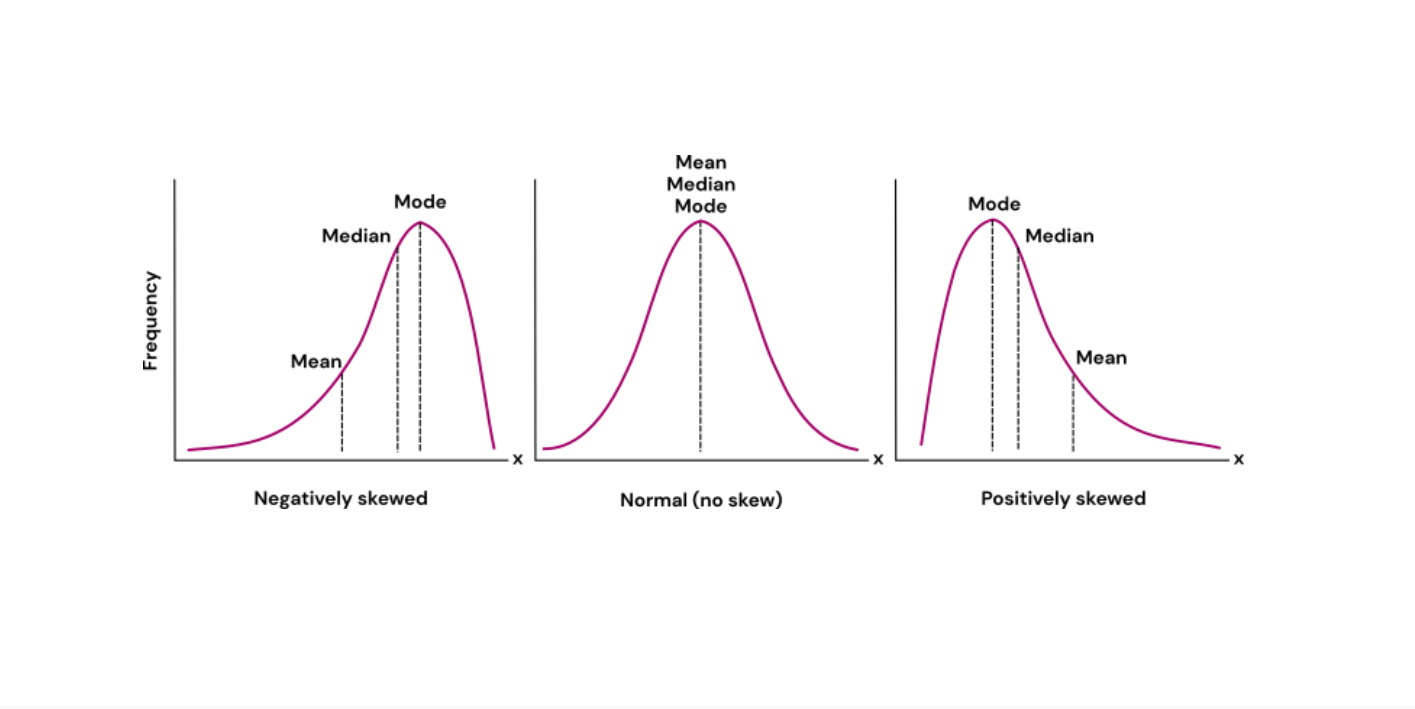
\includegraphics[scale=0.2]{figs/medidas_centralidade.png}
		\end{figure}
	\end{block}
\end{frame}

\begin{frame}{}
	\frametitle{}
	\begin{block}{}
		\justifying
		\begin{figure}[h]
			\centering
			\caption{Visualização Geométrica da moda, média e mediana de uma função densidade de probabilidade arbitrária}
			\begin{tikzpicture}[scale=1]
				\draw[line width=2, fill=green] (-4.9,1.7) .. controls (-4.2,2.4) and (-4.3,3.9) .. (-3.7,3.9) .. controls (-3,3.9) and (-2.5,2.3) .. (1.1,1.7) .. controls (-1,1.7) and (-2.1,1.7) .. (-4.9,1.7);
				\draw[line width=2] (-4.7,3.95) -- (-2.4,3.95);
				\draw[line width=2] (-3.7,3.95) -- (-3.7,1.2);
				\node at (-0.9,3.4) {\bf{Moda}};
				
				\draw[line width=2, fill=orange] (-4.9,-1.5) .. controls (-4.2,-0.8) and (-4.3,0.7) .. (-3.7,0.7) .. controls (-3,0.7) and (-2.5,-0.9) .. (1.1,-1.5) .. controls (-1,-1.5) and (-2.1,-1.5) .. (-4.9,-1.5);
				%\draw[line width=2] (-4.7,3.95) -- (-2.4,3.95);
				\draw[line width=2] (-2.8,0.5) -- (-2.8,-1.8);
				\node at (-3.5,-0.9) {\Large \bf{$50\%$}};
				\node at (-1.9,-0.9) {\Large \bf{$50\%$}};
				\node at (-0.9,0) {\bf{Mediana}};
				\draw[line width=2, fill=red] (2,0) .. controls (2.7,0.7) and (2.6,2.2) .. (3.2,2.2) .. controls (3.7,2.2) and (4.4,0.5) .. (8,0) .. controls (5.9,0) and (4.8,0) .. (2,0);
				%\draw[line width=2] (-4.7,3.95) -- (-2.4,3.95);
				\draw[line width=2] (-3.7,3.95) -- (-3.7,1.2);
				\draw[line width=2, fill=gray] (3.8,0) -- (3.3,-0.6) -- (4.3,-0.6) -- (3.8,0);
				\draw[line width=2] (3,-0.6) -- (4.6,-0.6);
				\draw[line width=1] (3.2,-0.6) -- (3,-0.8);
				\draw[line width=1] (3.4,-0.6) -- (3.2,-0.8);
				\draw[line width=1] (3.6,-0.6) -- (3.4,-0.8);
				\draw[line width=1] (3.8,-0.6) -- (3.6,-0.8);
				\draw[line width=1] (4,-0.6) -- (3.8,-0.8);
				\draw[line width=1] (4.2,-0.6) -- (4,-0.8);
				\draw[line width=1] (4.4,-0.6) -- (4.2,-0.8);
				\draw[line width=1] (4.6,-0.6) -- (4.4,-0.8);
				\draw (1.5,0.2) .. controls (1.3,0) and (1.3,-0.2) .. (1.5,-0.5);
				\draw (1.3,0.2) .. controls (1.1,0) and (1.1,-0.2) .. (1.3,-0.5);
				\draw (8.2,0.4) .. controls (8.4,0.2) and (8.4,-0.2) .. (8.3,-0.4);
				\draw (8.5,0.4) .. controls (8.7,0.2) and (8.7,-0.2) .. (8.6,-0.4);
				\node at (4.8,2) {\bf{Média}};
			\end{tikzpicture}
		\end{figure}
	\end{block}
\end{frame}

\section{Propriedades Importantes}
\subsection{Média Aritmética}
\begin{frame}{}
	\frametitle{}
	\begin{block}{Propriedade 1:}
		\justifying
		Sejam $X$ e $Y$ variáveis aleatórias e $k$ uma constante. Se $X=Y+k,$ então $\bar{X}=\bar{Y}+k$
	\end{block}
	\pause
	\begin{block}{Demonstração}
		\begin{minipage}{0.4\textwidth}
			\begin{align*}
				\bar{X}&=\dfrac{{\displaystyle \sum_{i=1}^{n}x_{i}}}{n}\\ 
				\vspace{0.1cm}
				&=\dfrac{x_{1}+\cdots+x_{n}}{n}\\ \vspace{0.1cm}
				&=\dfrac{(y_{1}+k)+\cdots+(y_{n}+k)}{n}\\
			\end{align*}
		\end{minipage}\pause\hfill
		\begin{minipage}{0.4\textwidth}
			\begin{align*}
				&=\dfrac{(y_{1}+\cdots+y_{n})+
					(k+\cdots+k)}{n}\\ \vspace{0.1cm}
				&=\dfrac{(y_{1}+\cdots+y_{n})+
					nk}{n}\\ \vspace{0.1cm}
				&=\dfrac{{\displaystyle \sum_{i=1}^{n}y_{i}}}{n}+k=\bar{Y}+k
			\end{align*}
		\end{minipage}
	\end{block}
\end{frame}

\begin{frame}{}
	\frametitle{}
	\begin{block}{Propriedade 2:}
		\justifying
		Sejam $X$ e $Z$ variáveis aleatórias e $k$ uma constante. Se $X=kZ,$ então $\bar{X}=k\bar{Z}$
	\end{block}
	\pause
	\begin{block}{Demonstração}
		\begin{minipage}{0.4\textwidth}
			\begin{align*}
				\bar{X}&=\dfrac{{\displaystyle \sum_{i=1}^{n}x_{i}}}{n}\\ 
				\vspace{0.1cm}
				&=\dfrac{x_{1}+\cdots+x_{n}}{n}\\ \vspace{0.1cm}
				&=\dfrac{(kz_{1})+\cdots+(kz_{n})}{n}\\
			\end{align*}
		\end{minipage}\pause\hfill
		\begin{minipage}{0.4\textwidth}
			\begin{align*}
				&=\dfrac{k(z_{1}+\cdots+z_{n})}{n}\\ \vspace{0.1cm}
				&=\dfrac{{\displaystyle k\sum_{i=1}^{n}z_{i}}}{n}=k\bar{Z}
			\end{align*}
		\end{minipage}
	\end{block}
\end{frame}

\begin{frame}{}
	\frametitle{}
	\begin{block}{Propriedade 3:}
		\justifying
		Seja $X$ uma variável aleatória qualquer. Considere $e_{i}=x_{i}-\bar{x}$ o i-ésimo desvio. Então $\sum_{i=1}^{n}e_{i}=0.$
	\end{block}
	\pause
	\begin{block}{Demonstração}
		\begin{minipage}{0.4\textwidth}
			\begin{align*}
				{\displaystyle \sum_{i=1}^{n}e_{i}}&=
				{\displaystyle \sum_{i=1}^{n}(x_{i}-\bar{x})}\\ 
				\vspace{0.1cm}
				&={\displaystyle \sum_{i=1}^{n}x_{i}-\sum_{i=1}^{n}\bar{x}}\\ \vspace{0.1cm}
				&={\displaystyle \sum_{i=1}^{n}x_{i}}-n\bar{x}\\
			\end{align*}
		\end{minipage}\pause\hfill
		\begin{minipage}{0.4\textwidth}
			\begin{align*}
				&={\displaystyle \sum_{i=1}^{n}x_{i}}-n \dfrac{{\displaystyle\sum_{i=1}^{n}x_{i}}}{n}\\ \vspace{0.1cm}
				&={\displaystyle \sum_{i=1}^{n}x_{i}}- {\displaystyle\sum_{i=1}^{n}x_{i}}\\ \vspace{0.1cm}
				&=0\\
			\end{align*}
		\end{minipage}
	\end{block}
\end{frame}

\subsection{Mediana}
\begin{frame}{}
	\frametitle{}
	\begin{block}{Propriedade 1:}
		\justifying
		Sejam $X$ e $Y$ variáveis aleatórias e $k$ uma constante. Se $X=Y+k,$ então $Md(X)=Md(Y)+k$
	\end{block}
	\pause
	\begin{block}{Propriedade 2:}
		\justifying
		Sejam $X$ e $Z$ variáveis aleatórias e $k$ uma constante. Se $X=kZ,$ então $Md(X)=kMd(Z)$
	\end{block}
\end{frame}

\subsection{Moda}
\begin{frame}{}
	\frametitle{}
	\begin{block}{Propriedade 1:}
		\justifying
		Sejam $X$ e $Y$ variáveis aleatórias e $k$ uma constante. Se $X=Y+k,$ então $Mo(X)=Mo(Y)+k$
	\end{block}
	\pause
	\begin{block}{Propriedade 2:}
		\justifying
		Sejam $X$ e $Z$ variáveis aleatórias e $k$ uma constante. Se $X=kZ,$ então $Mo(X)=kMo(Z)$
		\nocite{Morettin09} \nocite{eric}
	\end{block}
\end{frame}

\begin{frame}{}
	\frametitle{Observação Importante}
	\begin{block}{}
		\justifying
		Lembre-se: \textbf{a mediana é mais robusta que a média} em situações com valores muito extremos (outliers). Por isso, sempre avalie qual medida de posição faz mais sentido para o conjunto de dados que você está analisando!
	\end{block}
\end{frame}





\begin{frame}[allowframebreaks]
\frametitle{\bf Referências}
\printbibliography[heading=none]
\end{frame}



\end{document}
